\documentclass[11pt,]{article}
\usepackage{lmodern}
\usepackage{amssymb,amsmath}
\usepackage{ifxetex,ifluatex}
\usepackage{fixltx2e} % provides \textsubscript
\ifnum 0\ifxetex 1\fi\ifluatex 1\fi=0 % if pdftex
  \usepackage[T1]{fontenc}
  \usepackage[utf8]{inputenc}
\else % if luatex or xelatex
  \ifxetex
    \usepackage{mathspec}
  \else
    \usepackage{fontspec}
  \fi
  \defaultfontfeatures{Ligatures=TeX,Scale=MatchLowercase}
  \newcommand{\euro}{€}
\fi
% use upquote if available, for straight quotes in verbatim environments
\IfFileExists{upquote.sty}{\usepackage{upquote}}{}
% use microtype if available
\IfFileExists{microtype.sty}{%
\usepackage{microtype}
\UseMicrotypeSet[protrusion]{basicmath} % disable protrusion for tt fonts
}{}
\usepackage[margin=1in]{geometry}
\usepackage{hyperref}
\PassOptionsToPackage{usenames,dvipsnames}{color} % color is loaded by hyperref
\hypersetup{unicode=true,
            pdfborder={0 0 0},
            breaklinks=true}
\urlstyle{same}  % don't use monospace font for urls
\usepackage{graphicx,grffile}
\makeatletter
\def\maxwidth{\ifdim\Gin@nat@width>\linewidth\linewidth\else\Gin@nat@width\fi}
\def\maxheight{\ifdim\Gin@nat@height>\textheight\textheight\else\Gin@nat@height\fi}
\makeatother
% Scale images if necessary, so that they will not overflow the page
% margins by default, and it is still possible to overwrite the defaults
% using explicit options in \includegraphics[width, height, ...]{}
\setkeys{Gin}{width=\maxwidth,height=\maxheight,keepaspectratio}
\setlength{\parindent}{0pt}
\setlength{\parskip}{6pt plus 2pt minus 1pt}
\setlength{\emergencystretch}{3em}  % prevent overfull lines
\providecommand{\tightlist}{%
  \setlength{\itemsep}{0pt}\setlength{\parskip}{0pt}}
\setcounter{secnumdepth}{0}

%%% Use protect on footnotes to avoid problems with footnotes in titles
\let\rmarkdownfootnote\footnote%
\def\footnote{\protect\rmarkdownfootnote}

%%% Change title format to be more compact
\usepackage{titling}

% Create subtitle command for use in maketitle
\newcommand{\subtitle}[1]{
  \posttitle{
    \begin{center}\large#1\end{center}
    }
}

\setlength{\droptitle}{-2em}
  \title{}
  \pretitle{\vspace{\droptitle}}
  \posttitle{}
  \author{}
  \preauthor{}\postauthor{}
  \date{}
  \predate{}\postdate{}


% load packages
\usepackage{amsmath,amsfonts,float,makecell,titletoc,tocloft,titlesec,natbib,pdfpages,lineno,booktabs}
\usepackage[T1]{fontenc}
\usepackage{lmodern}
\usepackage[utf8]{inputenc}
\usepackage[doublespacing]{setspace}

% format captions
\usepackage[labelfont={small,bf}, labelsep=space, font={small}]{caption}

% format headings
\titleformat{\subsection}
{\normalfont\Large\bfseries}{\thesubsection}{1em}{}
\titleformat{\subsubsection}
{\normalfont\large\bfseries}{\thesubsubsection}{1em}{}
\titleformat{\paragraph}
{\normalfont\normalsize\bfseries}{\theparagraph}{1em}{}
\titleformat{\subparagraph}
{\normalfont\normalsize\itshape}{\thesubparagraph}{1em}{}

\titlespacing\paragraph{0pt}{12pt plus 4pt minus 2pt}{+0pt plus 2pt minus 2pt}
\titlespacing{\subparagraph}{0pt}{6pt plus 4pt minus 2pt}{+0pt plus 2pt minus 2pt}

% format toc
\renewcommand\cftsubsecfont{\normalfont\normalsize\bfseries}
% \renewcommand\cftsubsubsecfont{\normalfont\normalsize\bfseries}
% \renewcommand\cftparafont{\normalfont\normalsize\bfseries}
% \renewcommand\cftsubparafont{\normalfont\normalsize\itshape}

% make figures static
\let\origfigure\figure
\let\endorigfigure\endfigure
\renewenvironment{figure}[1][2] {
	\expandafter\origfigure\expandafter[H]
} {
	\endorigfigure
}

% define struts for tables
\newcommand\T{\rule{0pt}{2.6ex}} % top strut
\newcommand\B{\rule[-1.2ex]{0pt}{0pt}} % bottom strut

% define command to put new lines in table cells
%\newcommand{\specialcell}[2][c]{%
%  \begin{tabular}[#1]{@{}c@{}}#2\end{tabular}}
% insert S before figure and table caption
\pagenumbering{gobble}

% Redefines (sub)paragraphs to behave more like sections
\ifx\paragraph\undefined\else
\let\oldparagraph\paragraph
\renewcommand{\paragraph}[1]{\oldparagraph{#1}\mbox{}}
\fi
\ifx\subparagraph\undefined\else
\let\oldsubparagraph\subparagraph
\renewcommand{\subparagraph}[1]{\oldsubparagraph{#1}\mbox{}}
\fi

\begin{document}

\subsection{Figures}\label{figures}

\begin{figure}[htbp]
\centering
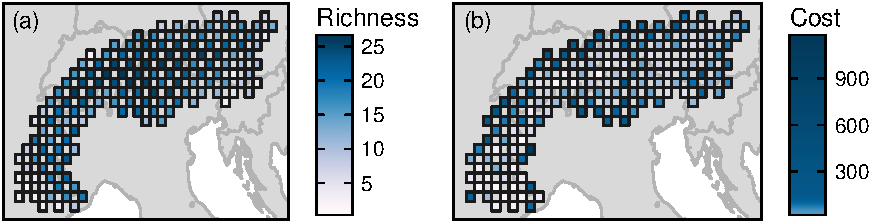
\includegraphics{figures_files/figure-latex/unnamed-chunk-3-1.pdf}
\caption{Map of the study area. Squares denote planning units. Panel (a)
depicts patterns of species riches. Planning units with a brighter color
are inhabited by more species. Panel (b) shows the distribution of
opportunity cost across the study area (computed as total population
density). Note that a quantile-based color ramp is used in this panel.}
\end{figure}

\begin{figure}[htbp]
\centering
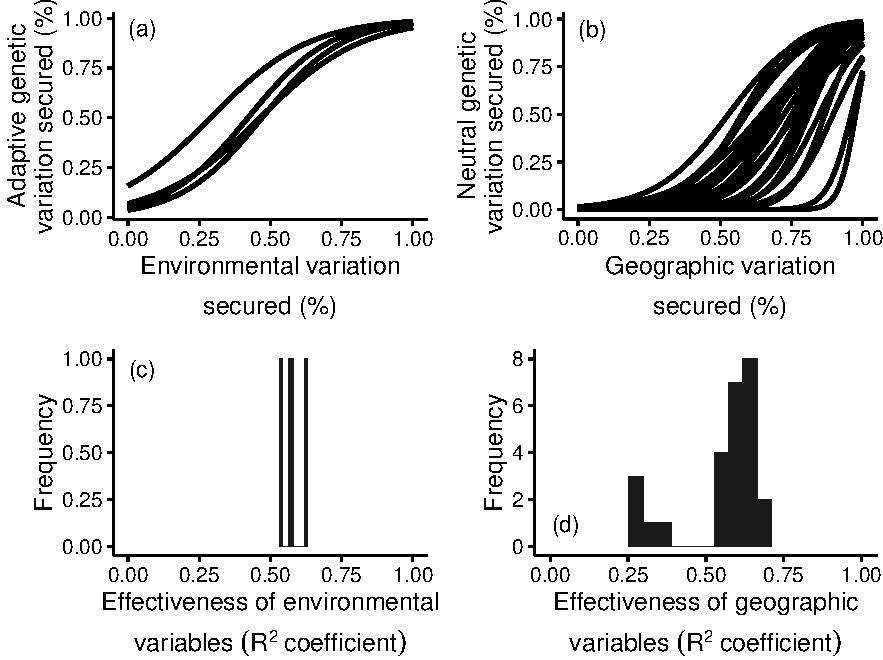
\includegraphics{figures_files/figure-latex/unnamed-chunk-4-1.pdf}
\caption{The relationship between surrogates and genetic variation
secured in prioritizations. Panel (a) shows the relationship between the
proportion of intra-specific adaptive genetic variation and
environmental variation secured in a prioritization. Similarly, panel
(b) shows the relationship between the proportion of intra-specific
neutral variaiton and geograpgic variation secured in a prioritization.
Panels (c) and (d) show the distribution of \(R^2\) values for these
models.}
\end{figure}

\begin{figure}[htbp]
\centering
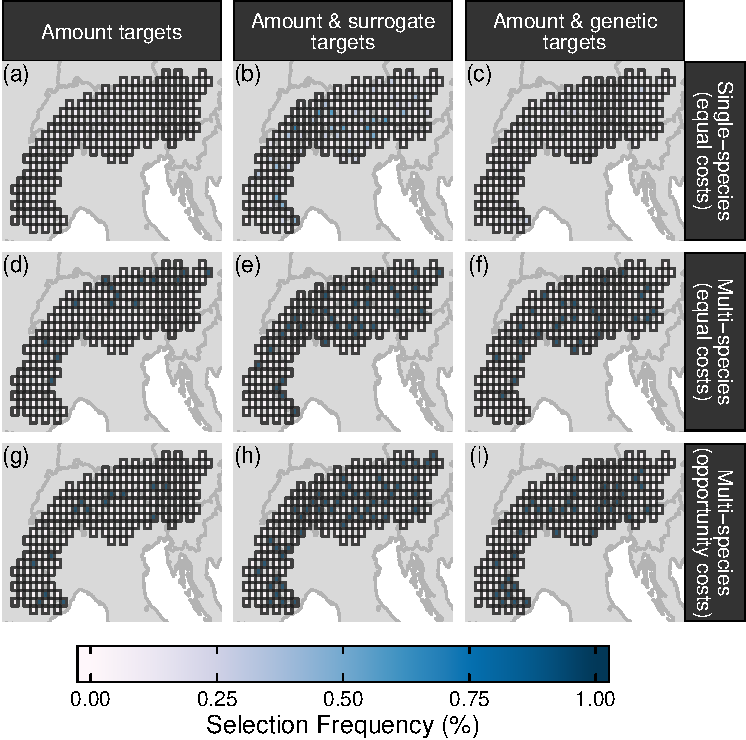
\includegraphics{figures_files/figure-latex/unnamed-chunk-5-1.pdf}
\caption{Planning unit selection frequencies. The top row of panels (a,
b, c) show single-species prioritizations generated assuming equal
costs. The middle row of panels (d, e, f) show multi-species
prioritizations generated assuming equal costs. The bottom row of panels
(g, h, i) show multi-species generated using opportunity costs. The left
column of panels (a, d, g) show prioritizations generated using only
amount-based targets. The middle column of panels (b, e, h) show
prioritizations generated using amount- and surrogate-based targets. The
right column of panels (c, f, i) show prioritizations generated using
amount- and genetic-based targets.}
\end{figure}

\begin{figure}[htbp]
\centering
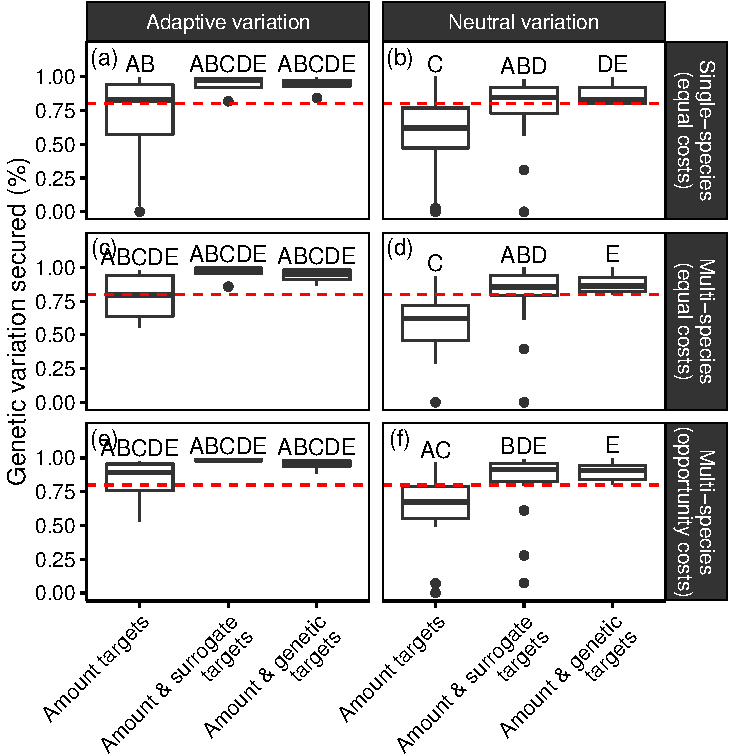
\includegraphics{figures_files/figure-latex/unnamed-chunk-6-1.pdf}
\caption{The effectiveness of prioritizations at securing genetic
variation. The top row of panels (a--b) show the performance of
single-species prioritizations generated assuming equal costs among
planning costs. The middle row of panels (c--d) show the performance of
multi-species prioritizations generated assuming equal costs among
planning units. The bottom row of panels (e--f) show the performance of
multi-species prioritizations generated using opportunity costs. The
left column of panels (a, c, d) and the right column of panels (b, d, f)
show the proportion of adaptive and neutral genetic variation secured
(respectively). Box plots show the effectiveness of prioritizations
generated using amount-based targets, amount-based and surrogate-based
targets, and amount-based and genetic-based targets for each species.
Letters denote significant differences (\(P < 0.05\)).}
\end{figure}

\hypertarget{refs}{}

\end{document}
